\documentclass[a4paper,12pt]{report}
\usepackage{amssymb}
\usepackage{amsmath}
\usepackage{amsthm}
\usepackage{amsfonts}
\usepackage{mathrsfs}
\usepackage{tikz}
\usetikzlibrary{arrows,automata}
\usepackage{color}
\usepackage[cm-default]{fontspec}
\usepackage{xunicode}
\usepackage{xltxtra}
\usepackage[all,cmtip]{xy}
\usepackage{xgreek}

\usepackage{algpseudocode}
\usepackage{algorithm}
\usepackage{minted}


\setmainfont[Mapping=tex-text]{GFS Neohellenic}

\title{ Αλγόριθμοι και Πολυπλοκότητα \\ 3η Σειρά Γραπτών Ασκήσεων}
\author{Γιαννέλος Γιάννης\\ΑΜ:03108088}

\begin{document}
\maketitle

\section*{Άσκηση 1: Προβολή ταινιών}
Για την επίλυση αυτού του προβλήματος θα εργαστούμε ως εξής. Θα αποθηκεύσουμε για κάθε ταινία την πληροφορία για το αν η ταινία είναι επιλεγμένη ή όχι απο τον χρήστη. Ακόμα θα χρειαστούμε την πληροφορία για το αν η ταινία είναι επιλεγμένη για το Σάββατο ή την Κυριακή, αυξάνοντας κάθε φορά εναν απο δύο κατάλληλους μετρητές σύμφωνα με τις επιλογές του χρήστη. Έχοντας λάβει υπόψη μας όλα τα δεδομένα για κάθε χρήστη, προγραμματίζουμε την προβολή της ταινίας (αν έχει επιλεχθεί απο κάποιον) την μέρα που μας δείχνει ο αντίστοιχος μετρητής. Σε περίπτωση που μια ταινία δεν έχει επιλεχθεί απο κανέναν, δεν την προγραμματίζουμε για προβολή και σε περίπτωση που οι μετρητές δείχνουν τον ίδιο αριθμό για Σάββατο και Κυριακή δεν μας νοιάζει ποια μέρα θα προβληθεί.   

\section*{Άσκηση 2: Μέτρηση συντομότερων μονοπατιών}
Ο υπολογισμός όλων των συντομότερων μονοπατιών, σε ένα γράφο $G(V,E)$ με μοναδιαία μήκη ακμών, μεταξύ δύο κορυφών $s-t$, $s,t \in V$, θα μπορούσε να γίνει με μια τροποποίηση στον αλγόριθμο Breadth First Search. Τα βήματα που θα ακολουθήσουμε θα είναι τα εξής:
\begin{itemize}
 \item Ξεκινάμε απο την κορυφή $s$ και την μαρκάρουμε ως ``υπο εξέταση''.
 \item Θεωρούμε τον κόμβο $s$ ``εξερευνημένο`` και κάθε γειτονική κορυφή του $s$ την μαρκάρουμε ως ``υπο εξέταση''.
 \item Θέτουμε την τρέχουσα κορυφή ``εξερευνημένη`` και επαναλαμβάνουμε την παραπάνω διαδικασία αγνωόντας τις ήδη εξερευνημένες.
 \item Mόλις βρούμε την κορυφή $t$ για πρώτη φόρα, σταματάμε την διαδικασία και επαναλαμβάνουμε τα παραπάνω στις ανεξερεύνητες κορυφές.
 \item Ο αριθμός των συντομότερων μονοπατιών είναι αριθμός που βρίσκουμε το $t$ μέχρι το τέλος της εκτέλεσης του παραπάνω αλγορίθμου. 
\end{itemize}
O αλγόριθμος έχει πολυπλοκότητα $O(n)$     

\section*{Άσκηση 3: Ελάχιστο συνδετικό δέντρο υπο περιορισμούς}
\subsection*{(α) Παραδείγματα γράφων}
\begin{itemize}
 \item Αρχικός γράφος: 
  \begin{center}
    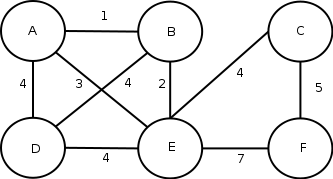
\includegraphics[scale=0.5]{./files/ex3-graph.png}
  \end{center}
 \item Minimum spanning tree: 
  \begin{center}
    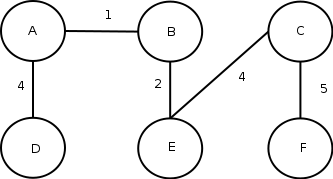
\includegraphics[scale=0.5]{./files/ex3-alt-mst.png}
  \end{center}
 \item Minimum spanning tree θεωρώντας L τις κορυφές A-D: 
  \begin{center}
    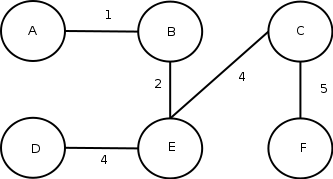
\includegraphics[scale=0.5]{./files/ex3-mst.png}
  \end{center}
\end{itemize}

\subsection*{(β) Αλγόριθμος MST με περιορισμούς}
Για να κατασκευάσουμε το ελάχιστο συνδετικό δέντρο με τους περιορισμούς που έχουν δωθεί (κορυφές υπογράφου να είναι φύλλα του MST) θα εργαστούμε ως εξής. Αρχικα θα αφαιρέσουμε τον υπογράφο απο τον αρχικό γράφο και θα βρούμε με την χρήση του αλγορίθμου Prim ή Kruskal ένα ενδιάμεσο ελάχιστο συνδετικό δέντρο. Στη συνέχεια προσθέτουμε τις κορυφές που είχαμε αφαιρέσει στο ελάχιστο συνδετικό δέντρο (που θα είναι πλεόν σίγουρα φύλλα) και θα εκτελέσουμε ξανά έναν εκ των δυο αλγορίθμων για την εύρεση του ελάχιστου συνδετικού δέντρου (Prim ή Kruskal) για να παράγουμε το ζητούμενο MST με τους κατάλληλους περιορισμούς.

\section*{Άσκηση 4: Μοναδικότητα ελάχιστου συνδετικού δέντρου}
\subsection*{(α) Παράδειγμα}
\begin{itemize}
 \item Αρχικός γράφος:
\begin{center}
 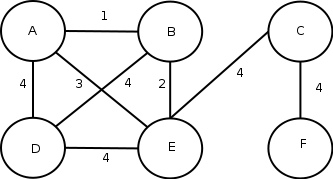
\includegraphics[scale=0.5]{./files/ex4-graph.png}
\end{center}
 \item Mοναδικό MST:
\begin{center}
 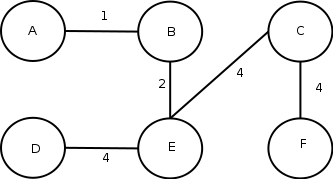
\includegraphics[scale=0.5]{./files/ex4-mst.png}
\end{center}
\end{itemize}

\subsection*{(γ) Συνθήκη για μοναδικότητα MST}
\begin{itemize}
 \item \textbf{Συνθήκη:} \textit{Αν κάθε ακμή έχει μοναδικό βάρος τότε υπάρχει μοναδικό ελάχιστο συνδετικό δέντρο}
 \item \textbf{Απόδειξη:} Έστω Α ελάχιστο συνδετικό δέντρο το οποίο δεν είναι μοναδικό. Τότε υπάρχει άλλο ελάχιστο συνδετικό δέντρο με ίδιο βάρος, έστω B. Έστω $e_1$ ακμή που έιναι στο A και όχι στο B. Αφού το B είναι ελάχιστο συνδετικό δέντρο, τo $\{e_1\}\bigcup B$ θα πρέπει να περιέχει κύκλο C. Ακόμα στο Β θα πρέπει να υπάρχει ακμή $e_2$ η οποία δεν είναι στον A και είναι στον κύκλο C. Έστω ότι το βάρος της ακμής $e_1$ είναι μικρότερο απο το βάρος της $e_2$. Αν αντικαταστήσουμε την $e_2$ με την $e_1$ στον Β, προκύπτει ένα ελάχιστο συνδετικό δέντρο $\{e_1\} \bigcup B - \{e_2\} $ το οποίο έχει μικρότερο βάρος απο το B. \textbf{ΑΤΟΠΟ}  
\end{itemize}


\end{document}
